\documentclass[aps,pre,twocolumn,letterpaper,floatfix]{revtex4}
\usepackage{graphicx} 
\usepackage{amsmath,amssymb,amsfonts} 
\usepackage{mathtools}
\usepackage{pdfpages}
\usepackage{afterpage}
\usepackage{todo}
\usepackage[hidelinks]{hyperref} 
\usepackage{epstopdf}
\begin{document}
\title{Atomify - a live LAMMPS visualizer}
\author{Anders Hafreager$^1$}
\author{Svenn-Arne Dragly$^{1}$}
\affiliation{$^1$Department of Physics - University of Oslo\\Sem S{\ae}lands vei 24, NO-0316, Oslo, Norway }
\date{\today} 

%%%%%%%%%%%%%%%%%%%%%%%%%%%%%%%%%%%%%%%%%%%%%%%%%%%%%%%%%%%%%%
%%%%%%%%%%%%%%%%%%%%%%%%%%%%%%%%%%%%%%%%%%%%%%%%%%%%%%%%%%%%%%
\begin{abstract} 
The typical workflow when developing LAMMPS scripts includes working with several programs. A text editor is needed to modify the scripts, the terminal to run the simulation, and programs like VMD or Ovito to visualize the system over time. If physical quantities are computed, the data is often plotted with MATLAB or Python, where additional scripts must be used. This is a tedious process, especially for teaching purposes and for people who are new to LAMMPS. 
We here introduce Atomify; a high performance live visualizer for LAMMPS simulations, with stunning graphics able to simulate and render more than 250000 atoms with excellent frame rate on modern hardware. Atomify supports OpenMP acceleration, live plotting of LAMMPS variables and computes, and an easy-to-use code editor in one single program. Direct access to the powerful machinery already built into LAMMPS allows easy access to advanced physical quantities. Atomify is open source software (GPL) written in C++, built on top of Qt. 
\end{abstract} 
 
\maketitle
 
% %%%%%%%%%%%%%%%%%%%%%%%%%%%%%%%%%%%%%%%%%%%%%%%%%%%%%%%%%%%%%
%% %%%%%%%%%%%%%%%%%%%%%%%%%%%%%%%%%%%%%%%%%%%%%%%%%%%%%%%%%%%%
\section{Introduction}
Molecular dynamics (MD) has become a standard technique for simulating atoms and molecules in a broad range of fields. Over the years, increasingly sophisticated methods have been developed. With the large number of force fields, advanced techniques and GPU acceleration, implementing a good molecular dynamics program from scratch a challenging task. While many people at some point write their own MD code, most end up using one of the many available codes\footnote{See \url{https://en.wikipedia.org/wiki/Comparison_of_software_for_molecular_mechanics_modeling}} such as LAMMPS\cite{Plimpton1995Fast}, GROMACS\cite{Pronk2013}, NAMD\cite{Phillips2005Scalable}. These codes have been developed for more than two decades and contains more than one million lines of code each. \todo{check this}

The work in this paper is focused on LAMMPS. Although the software is well-documented and enables the user to perform advanced simulations, it can be a demanding job to learn how to use it well. A LAMMPS simulation is performed by a series of commands which are executed one by one. Physical quantities such as energy, temperature and stress can be measured by adding \textit{computes}. A time evolution of these quantities can in turn be saved to file for plotting and further analysis. Particle trajectories can be saved to a file and visualized by tools such as VMD\cite{Humphrey1996Vmd} or OVITO\cite{Stukowski2009Visualization}. The lack of an intuitive GUI and visualization \footnote{which are listed in the non-features list on the web page: \url{http://lammps.sandia.gov/non_features.html}} makes the workflow somewhat complicated. 

Atomify solves this problem by combining the script editing, simulating, visualizing and analyzing into one single application. It uses LAMMPS as a library and synchronizes after each timestep, copying the relevant information from LAMMPS to the GPU for visualization and data plotting. The visualization is done using raytracing on billboards allowing rendering of millions of atoms with good framerate. Atomify is designed with simplicity as main goal.

\todo{Write about existing GUI software such as Materials Studio and MacroModel}
\section{Features}
Atomify comes with many useful features in addition to the 
\subsection{Script editor}
The script editor is minimalistic with line numbers and syntax highlighting for the LAMMPS scripting language. It supports multiple open files and remembers which files you have open across working sessions. A simple Ctrl+R will restart the simulation with any changes you might have done.
\subsection{Visualization}
Visualization of the atomic positions and the molecular structure is done using very efficient billboard rendering using OpenGL and Qt 3D. 

\subsection{Group and region highlighting}


\subsection{Live plotting and property coloring}
LAMMPS can produce many different outputs using computes and variables. All computes, variables and fixes Time evolution of scalar quantities such as temperature, stress components and mean square displacement are 

If a compute or variable produces a per-atom quantity, it can be used to color the atoms on a color scale from the minimum finite value to the maximum finite value, see figure \ref{fig:property_coloring}. 

\begin{figure}
	\centering
	\includegraphics[width=0.5\textwidth]{property_coloring.png}
	\caption{Atomify can use any per-atom quantity to color the atoms through computes or variables. Here the atoms are colored using the velocity squared where the middle atoms have lower mass than the other atoms. }
	\label{fig:property_coloring}
\end{figure}

\section{Implementation}
Atomify is built upon Qt. All GUI is defined in QML whereas the backend of the program communicating with LAMMPS is written in c++. Simply put, Atomify runs an instance of a LAMMPS object enabling the user to visualize the current state of LAMMPS and interact with LAMMPS while the simulation is running. 

\subsection{Communicating with LAMMPS}
LAMMPS can be compiled as a library with most of its contents being accessable through either the library interface or public variables in all classes. 

\subsection{Live plotting}

\subsection{Data pipeline}
When rendering one often wants to modify the data from LAMMPS before it is visualized. Examples are periodic images of the simulation, slicing and coloring. We have been inspired by the pipeline used in Ovito where the data flows through several \textit{modifiers}, each modifying the visualization data before the data is converted to a format for the GPU.

\section{Rendering techniques}
Simulations of atoms are often visualized using spheres as atoms and cylinders. The spheres represent the atoms while the cylinders represent the bonds between the atoms. This way, the molecular structure is easy to understand and interpret. In many visualization tools, the spheres and cylinders are built up by many triangles connected so they form the geometrical object of interest. One problem with this rendering technique is that each sphere needs many, often hundreds, triangles in order to look spherical. This significantly reduces the rendering performance. A common technique to overcome this problem is to use billboards. Billboards are planes, made up by two or four triangles\footnote{The spheres are using two triangles, whereas the cylinders use four.} with surface normals parallel to the vector pointing towards the camera. By doing proper shading, the billboards can mimick the spheres and cylinders so they look realistic, see Figure \ref{fig:final_billboards}.

\begin{figure}
	\centering
	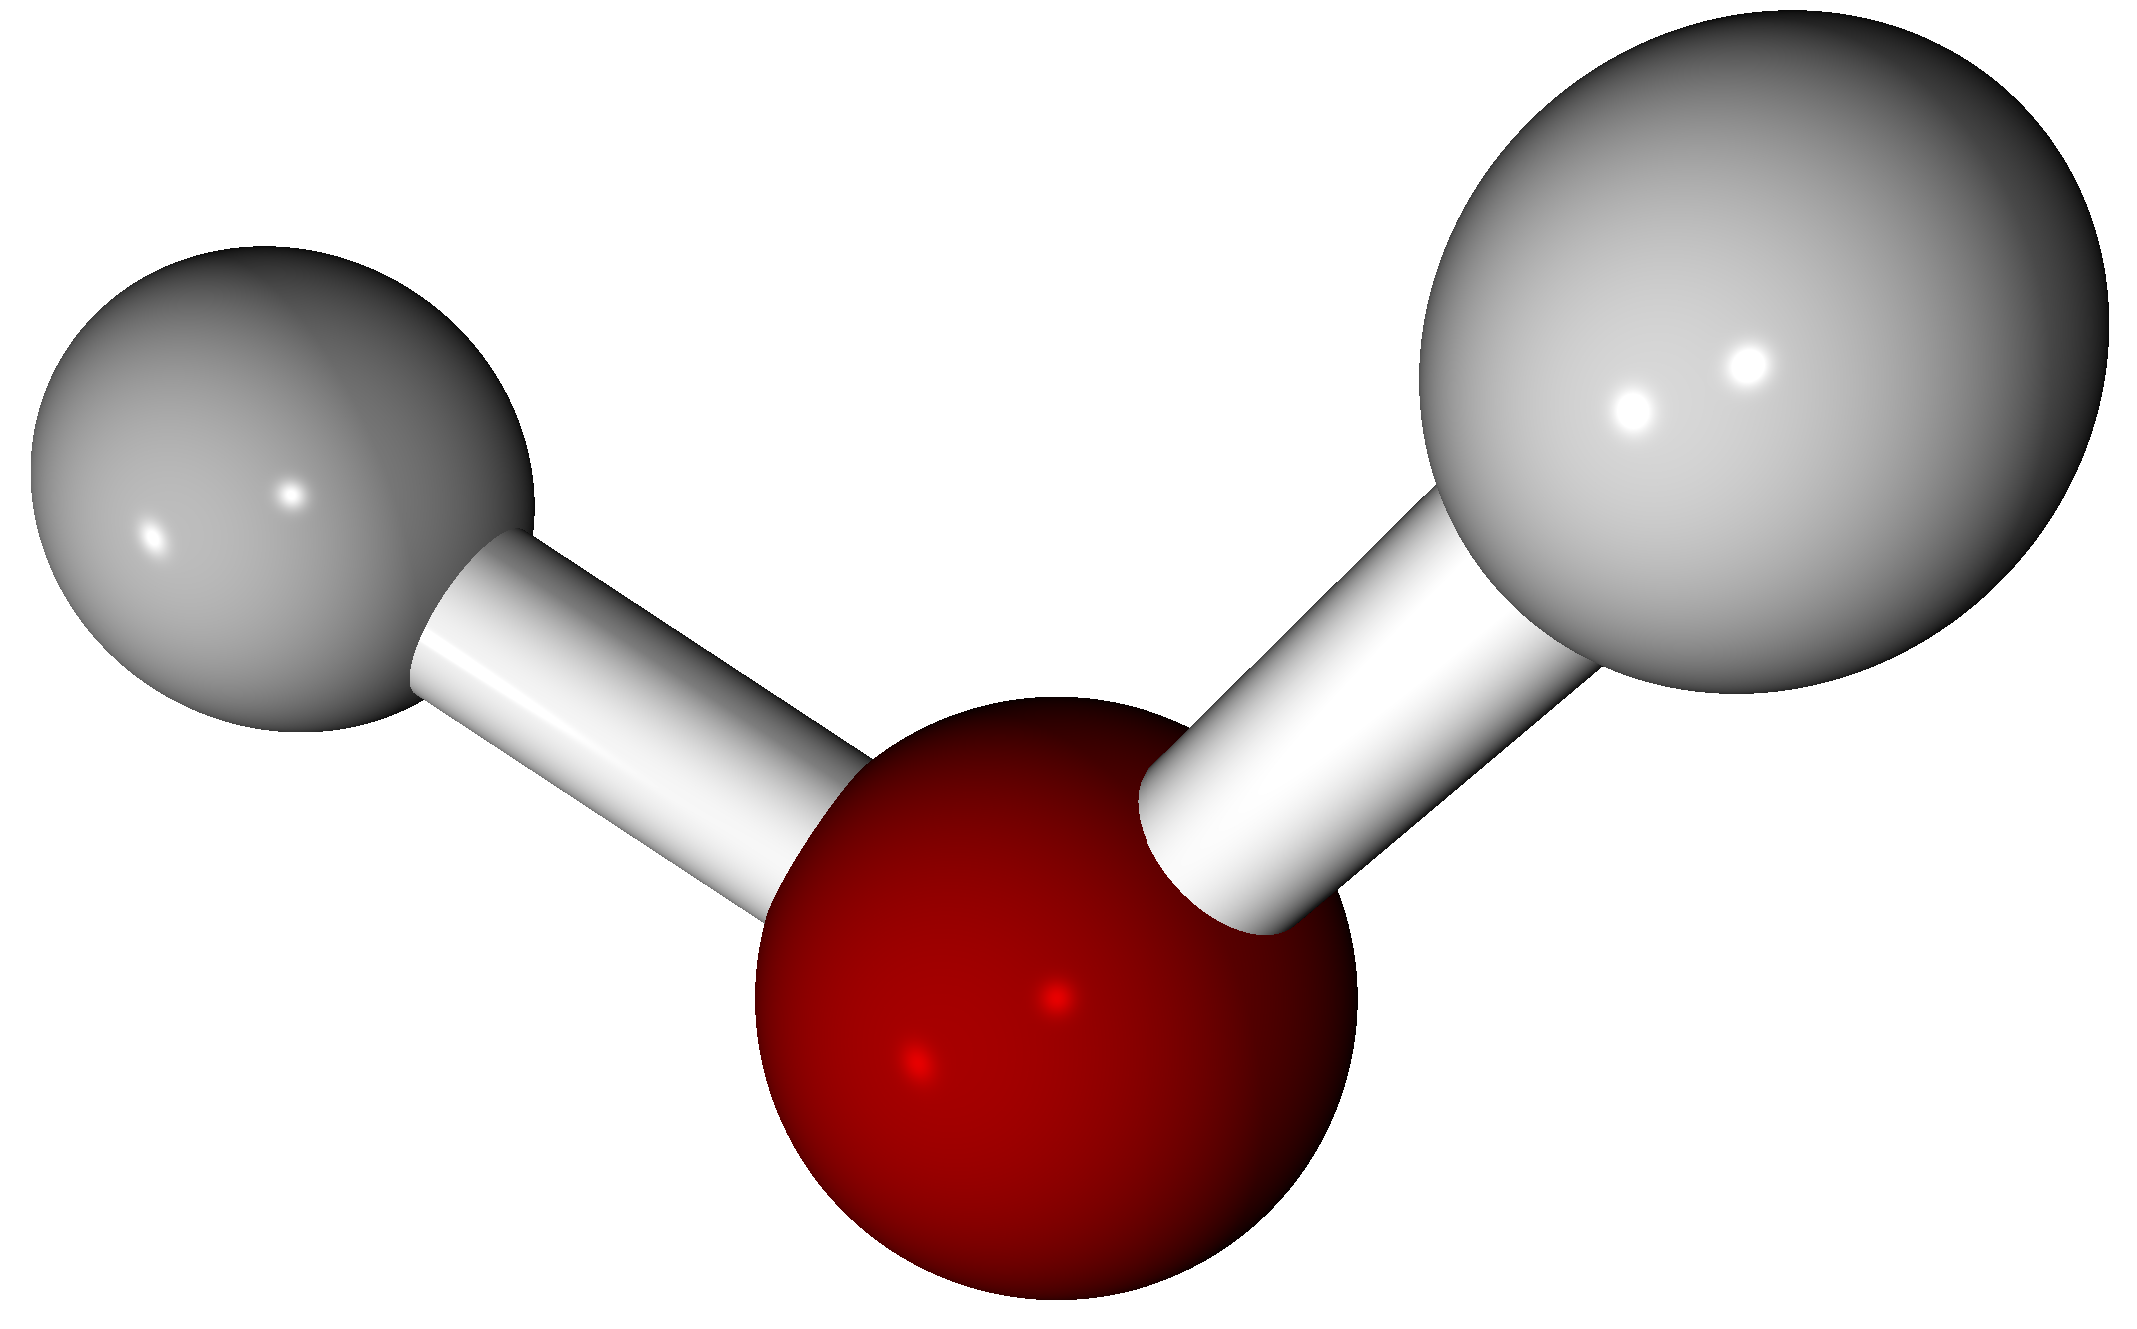
\includegraphics[width=0.5\textwidth]{final_billboard.png}
	\caption{Billboards can produce pixel perfect rendering of molecules. Here we see a water molecule being rendered as billboards with two light sources showing specular reflection and diffuse light effects. }
	\label{fig:final_billboards}
\end{figure}

\subsection{Sphere billboards}
Each sphere is visualized as two triangles making up a square large enough to cover all pixels the sphere needs. To reduce the CPU workload, all 4 corner vertices of the square are placed at the exact position of the sphere. The radius and a vertex id is specified, so that the vertex shader can move the 4 vertices so that the plane is orthogonal to the view vector and is larger than the cross sectional area of the sphere of interest. This is illustrated in figure \ref{fig:billboards}.

\begin{figure}
	\centering
	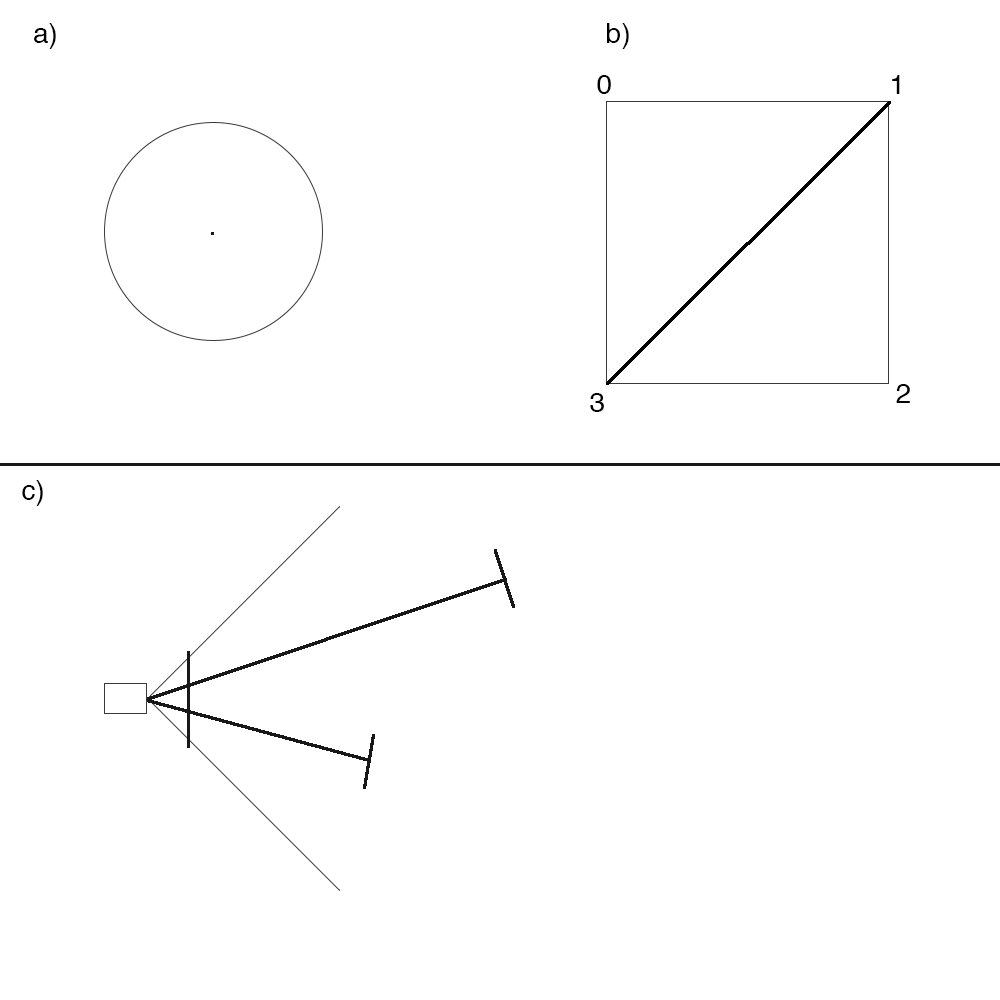
\includegraphics[width=0.5\textwidth]{spherebillboards.png}
	\caption{Illustration of billboards. The circles are shown in the figure to show our target rendering. a) all 4 vertices are at the center of the sphere. b) the vertex shader moves each vertex so that the plane covers a larger cross sectional area than the sphere. c) the orientation of the plane is such that the normal vector of the plane is parallel to the view vector. }
	\label{fig:billboards}
\end{figure}



\subsection{Cylinder billboards}
The cylinders are a bit more difficult because of two reasons. 
since they intersect with the spheres at the surface. This is solved by 

\section{Case study}
% Rerun on large dataset

\section{Conclusion}
We have

\subsection{Future work}
Atomify is far from finished.\\
A web version of Atomify is in development using WebGL and Emscripten. \\
Geometry shaders \\
Improved script editor with auto completion \\
Moltemplate interface \\

\section{Availability}

\section{Acknowledgments}

\bibliographystyle{plain}
\bibliography{Remote}

\end{document}  